\subsection{Pearson Correlation}\label{subsec:pearsoncorrelation}

In order to test the validity of our metrics and the chosen policy, a pearson correlation between the metrics have been conducted. The pearson correlation is calculated on the scores of the metrics on the given trips. The point of the test is to make sure no metrics are directly correlating, meaning one of the metrics is negligible. There is a number of different reasons as to why the outcome will look as it does, and it will be discussed thoroughly.

The matrix of pearson correlations between the metrics is shown in Table \ref{tab:pearsonmatrix}. The most notable result is the multicollinearity between accelerations and brakes, which seems rather odd as they are diametrical opposites and can per definition not exist at the same time. Another highly correlating metric is jerks, having a correlation of 0.828 with both brakes and accelerations. 

\begin{table*}[tb]
\centering
\caption{This is the pearson correlation matrix between the metrics}
\label{tab:pearsonmatrix}
\begin{tabular}{|l|llllll|}
\hline
\rowcolor{tablegreen}
                      & Roadtypes & Critical Time Periods & Speeding & Accelerations & Brakes & Jerks \\\hline
Roadtypes             & 1 &  &  &  &  &  \\
Critical Time Periods & -0.250    & 1  &  &  &  &  \\
Speeding              & -0,546    & 0.156                 & 1  &  &  &  \\
Accelerations         & -0.341    & 0.460                 & 0.196    & 1  &  &   \\
Brakes                & -0,348    & 0.428                 & 0.195    & 0.971         & 1 &   \\
Jerks                 & -0,241    & 0.313                 & 0.144    & 0.828         & 0.828  & 1 \\\hline  
\end{tabular}
\end{table*}

Looking closer at the multicollinearity between accelerations and brakes, there are a couple of different factors which affect the result. As mentioned accelerating and braking are diametrically opposite, but they are both dependent on the speed of the vehicle (as they are calculated through the change in speed). If the driver performs a big acceleration, his speed is high and he, at some point, needs to brake in order to decline in speed. 

\begin{figure}[tb]
\centering
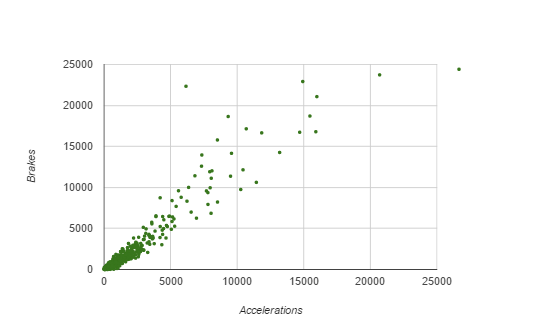
\includegraphics[width=0.465\textwidth]{Pictures/abcorrel}
\caption{A scatterplot of the correlation between acceleration- and brake score}
\label{fig:abcorrel}
\end{figure}

Figure \ref{fig:abcorrel} clearly illustrates the correlation between accelerations and brakes. Another reason as to why these metrics correlate can be the thresholds in the policy used to calculate the scores. As earlier mentioned the threshold for brakes are 8 $m/s^2$ whereas accelerations are counted from 5 $m/s^2$. If we had no thresholds and the delinquencies were scored the same, the correlation would be 1.0 as it only depended on the speed of the vehicle. 
Jerks was the metric that met the highest level of skepticism when the scoring model was designed, and the correlation shows that it was not completely unwarranted. It does show a lot of correlation with both brakes and accelerations. The figure \ref{fig:ajcorrel} shows the correlation between accelerations and jerks. Jerks are as mentioned calculated as $m/s^3$, and a driver with many accelerations are almost bound to have a lot of jerks as it is hard to keep a constant acceleration.

\begin{figure}[tb]
\centering
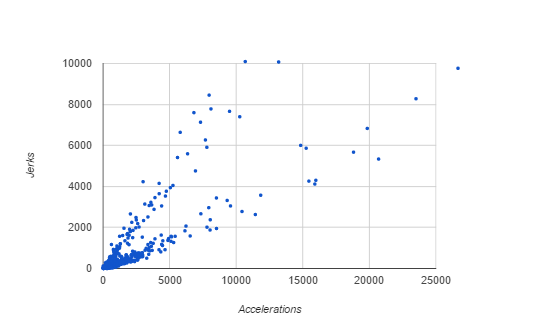
\includegraphics[width=0.465\textwidth]{Pictures/ajcorrel}
\caption{The correlation between acceleration- and jerk score}
\label{fig:ajcorrel}
\end{figure}


the similar correlation between the two can be answered by the correlation between accelerations and brakes. 
